\documentclass[a4paper]{article}
\usepackage{times}
\usepackage{mathptmx}
\usepackage[boldfont,slantfont]{xeCJK}
\setmainfont{Times New Roman}
\setsansfont{Times New Roman}
\setCJKmainfont{宋体}
\setCJKsansfont{黑体}
\setCJKmonofont{仿宋}
\setCJKfamilyfont{hei}{黑体}
\newcommand{\hei}{\CJKfamily{hei}}
\usepackage{amsmath,amssymb,amsthm}
\usepackage{geometry}
\geometry{left=2.5cm,right=2.5cm,top=2.5cm,bottom=2.5cm}
\usepackage{titlesec}
\titleformat{\section}{\Large \hei}{\thesection}{1em}{}
\titleformat{\subsection}{\large \hei}{\thesubsection}{1em}{}
\usepackage[colorlinks,linkcolor=black]{hyperref}
\usepackage{pgf,tikz}
\usetikzlibrary{calc,intersections}
\usetikzlibrary{arrows,snakes,backgrounds}
\usetikzlibrary{shapes.geometric}
\pgfmathdeclarefunction{fix}{1}{\global \pgfmathunitsdeclaredfalse}
\title{算法竞赛中的数学问题——例题}
\author{东北育才学校\quad 张听海}
\def\tcdots{\,\!\cdots\!\,}
\def\bkh{\!\!(}
\def\ekh{)\!\!}
\def\leq{\leqslant}
\def\geq{\geqslant}
\usepackage{indentfirst}
\begin{document}
    \renewcommand{\baselinestretch}{1.25}\normalsize
    \setlength{\parindent}{2em}
    \setlength{\abovedisplayskip}{1pt}
    \setlength{\belowdisplayskip}{1pt}
    \pagestyle{plain}

    \maketitle

    \tableofcontents

    \newpage

    \section{因数与倍数}

    \subsection{哈希函数}

    给定正整数$h$,\!\!求有多少对非负整数$(x,y)$满足$h=xy+x+y$.

    $T$组数据.

    $T\leq 10,000$,\!\!$h\leq {10}^8$.

    整理得$h+1=(x+1)(y+1)$. 即求$h+1$的正因子个数.

    欧拉筛预处理得到$1\sim {10}^4$之间的所有质数,\!\!进而得到$h+1$的质因子分解式.

    如果用所有找到的质数试除之后$h>1$,\!\!则剩下的$h$必为质数\bkh 即原$h$的最大质因子\ekh .

    注意到若$h+1=p_1^{\alpha_1}p_2^{\alpha_2}\cdots p_k^{\alpha_k}$,\!\!则$h+1$的正因子个数为$(\alpha_1+1)(\alpha_2+1)\cdots(\alpha_k+1)$.

    \subsection{[UOJ48]核聚变反应强度}

    给出$n$个正整数$a_1,a_2,\tcdots,a_n$,\!\!计算$a_1$与每个$a_i$的次大公约数\bkh 能同时整除$x,y$的正整数中第二大的数\ekh,\!\!如果没有输出$-1$.

    $n\leq {10}^5$,\!\!$a_i\leq {10}^{12}$.

    对于两个正整数$a_1$和$a_i$,\!\!它们的公约数必为$\gcd(a_1,a_i)$的公约数. 即求$\gcd(a_1,a_i)$的次大公约数.

    欧拉筛预处理出质数数列.

    对于每个$a_i$,\!\!欧几里得算法求出$\gcd(a_1,a_i)$,\!\!之后从小到大用质数试除,\!\!找到最小的$p\mid\gcd(a_1,a_i)$,\!\!输出$\dfrac{\gcd(a_1,a_i)}{p}$.

    \subsection{[BZOJ2299]向量}

    给你一对数$a,b$,\!\!你可以任意使用$(a,b),(a,-b),(-a,b),(-a,-b),(b,a),(b,-a),(-b,a),(-b,-a)$这些向量,\!\!问你能不能拼出另一个向量$(x,y)$.

    $T$组数据.

    $T\leq 50,000$,\!\!$-2\times {10}^9\leq a,b,x,y\leq 2\times {10}^9$.

    相当于有三种操作:\!\!

    $\bullet$给$x$或$y$加上或减去$2a$或$2b$.

    $\bullet$ {\ttfamily x=x+a,y=y+b}.

    $\bullet$ {\ttfamily x=x+b,y=y+a}.

    后两种操作可以使用0次或1次.

    枚举后两种操作是否使用,\!\!之后用裴蜀定理判定能否拼成.

    \subsection{[POJ3696] The Luckiest Number}

    对于给定的整数$L$,\!\!找出$L$能整除最短的全8序列的长度.

    注:\!\!全8序列为形如$\underbrace{888\cdots 8}_{n\text{个}8}$.

    多组数据.

    $1\leq L\leq 2\times {10}^9$.

    $\underbrace{888\cdots 8}_{n\text{个}8}=\dfrac{8}{9}\big({10}^n-1\big)=L\cdot p$,\!\!即${10}^x-1=\dfrac{9Lp}{8}$.

    设$m=\dfrac{9L}{\gcd(L,8)}$,\!\!则存在$p'$使得${10}^x-1=mp'$,\!\!即求${10}^x\equiv 1\pmod{m}$的最小解.

    当$\gcd(10,m)\neq 1$时,\!\!无解.

    当$\gcd(10,m)=1$时,\!\!由于${10}^{\varphi(m)}\equiv 1\pmod{m}$,\!\!只需考虑$\varphi(m)$的因子.

    对$\varphi(m)$质因数分解.

    对每个质因子$p_i$,\!\!执行$n=n/p_i$直到以下情形之一被满足:\!\!$(1)$ $p_i\nmid n$;\!\!$(2)$ $x^n\not\equiv 1\pmod{m}$.

    考虑过全部质因子后即得解.

    \section{欧拉函数}

    \subsection{[BZOJ2818] Gcd}

    给定整数$N$,\!\!求$1\leq x,y\leq N$且$\gcd(x,y)$为素数的数对$(x,y)$有多少对?

    $1\leq N\leq {10}^7$.

    欧拉筛法预处理质数数列及$\varphi(n)$前缀和.

    题目等价于求$1\leq x,y\leq\bigg\lfloor\dfrac{N}{p}\bigg\rfloor$且$\gcd(x,y)=1$的数对的个数,\!\!其中$p$为质数.

    \subsection{[BZOJ2190]仪仗队}

    一个$N\times N$的方阵,\!\!问从最后方的点能看到多少个点.

    \begin{center}
        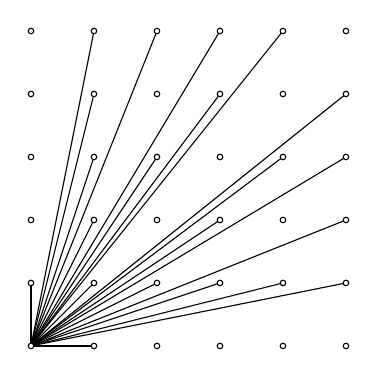
\begin{tikzpicture}[scale=0.8]
            \draw (0,0)--(1,0);
            \draw (0,0)--(0,1);
            \draw (0,0)--(1,1);
            \draw (0,0)--(2,1);
            \draw (0,0)--(3,1);
            \draw (0,0)--(4,1);
            \draw (0,0)--(5,1);
            \draw (0,0)--(1,2);
            \draw (0,0)--(3,2);
            \draw (0,0)--(5,2);
            \draw (0,0)--(1,3);
            \draw (0,0)--(2,3);
            \draw (0,0)--(4,3);
            \draw (0,0)--(5,3);
            \draw (0,0)--(1,4);
            \draw (0,0)--(3,4);
            \draw (0,0)--(5,4);
            \draw (0,0)--(1,5);
            \draw (0,0)--(2,5);
            \draw (0,0)--(3,5);
            \draw (0,0)--(4,5);
            \foreach \x in {0,1,...,5}
                \foreach \y in {0,1,...,5}
                    \draw [fill=white] (\x,\y) circle (1/0.8pt);
        \end{tikzpicture}
    \end{center}

    $1\leq N\leq 40,000$.

    满足以下情形之一的点可被看到:\!\!

    $(1)$该点为$(0,1),(1,0),(1,1)$之一;\!\!

    $(2)$ $2\leq x,y\leq n-1$且$\gcd(x,y)=1$.

    所求即$\displaystyle 3+\sum_{i=2}^{n-1}\varphi(i)$.

    欧拉筛求欧拉函数,\!\!求和.

    \subsection{[BZOJ3884]上帝与集合的正确用法}

    求$2^{2^{2^{2^{\cdots}}}}\bmod p$的值.

    $T$组数据.

    $T\leq 1,000$,\!\!$1\leq p\leq {10}^7$.

    欧拉筛预处理欧拉函数值.

    设$p=2^k\cdot q$,\!\!其中$q$为奇数. 则$2^{2^{2^{2^{\cdots}}}}\bmod p=2^k\bigg(2^{2^{2^{2^{\cdots}}}-k}\bmod q\bigg)$.

    由欧拉定理$2^k\bigg(2^{2^{2^{2^{\cdots}}}-k}\bmod q\bigg)=2^k\bigg[2^{\big(2^{2^{2^{\cdots}}}-k\big)\bmod\varphi(q)}\bmod q\bigg]$.

    递归计算,\!\!直至$q=1$.

    \subsection{离散对数问题}

    已知$a,b,n$,\!\!解同余方程$a^x\equiv b\pmod{n}$,\!\!其中$\gcd(a,n)=1$.

    由欧拉定理,\!\!$a^x\equiv a^{x+\varphi(n)}\pmod{n}$. 因此只需枚举$0\leq x<\varphi(n)$.
    
    分块优化. 设$x=p\big\lceil\varphi(n)\big\rceil-q$,\!\!这里$0<p,q\leq\lceil\varphi(n)\big\rceil$.

    则$a^{p\lceil\varphi(n)\rceil-q}\equiv b\pmod{n}$等价于$a^{p\lceil\varphi(n)\rceil}\equiv b\cdot a^q\pmod{n}$.

    枚举$0<q\leq\lceil\varphi(n)\big\rceil$,\!\!用hash表记录余数与$q$值的关系.

    再枚举$p$,\!\!找到使$x$最小的$p,q$.

    以上算法也被称为大步小步法$($BSGS$)$.

    \section{三分法}

    \subsection{[BZOJ1857]传送带}

    在二维平面上有两个线段型传送带$AB$和$CD$,\!\!小明在传送带$AB$上的速度为$P$,\!\!在传送带$CD$上的速度为$Q$,\!\!在平面其余位置的速度为$R$,\!\!求小明从$A$走到$B$需要的最短时间.

    $1\leq P,Q,R\leq 10$,\!\!各点坐标$\leq 1,000$.

    三分套三分.
\end{document}